%!TEX root = main.tex
\documentclass[conference, tikz]{IEEEtran}
\IEEEoverridecommandlockouts
% The preceding line is only needed to identify funding in the first footnote. If that is unneeded, please comment it out.

\usepackage{physics}
\usepackage{tikz}
\usepackage{tikz-3dplot}
\usepackage[outline]{contour} % glow around text
\usepackage{xcolor}
% Tikz styles
\colorlet{veccol}{green!50!black}
\colorlet{projcol}{blue!70!black}
\colorlet{myblue}{blue!80!black}
\colorlet{myred}{red!90!black}
\colorlet{mydarkblue}{blue!50!black}
\tikzset{>=latex} % for LaTeX arrow head
\tikzstyle{proj}=[projcol!80,line width=0.08] %very thin
\tikzstyle{area}=[draw=veccol,fill=veccol!80,fill opacity=0.6]
\tikzstyle{vector}=[-stealth,myblue,thick,line cap=round]
\tikzstyle{unit vector}=[->,veccol,thick,line cap=round]
\tikzstyle{dark unit vector}=[unit vector,veccol!70!black]
\usetikzlibrary{angles,quotes} % for pic (angle labels)
\contourlength{1.3pt}

\usepackage{caption}
\usepackage[labelsep=quad,indention=10pt]{subfig}
\usepackage{amsmath,amssymb,amsfonts}
\usepackage{algorithmic}
\usepackage{graphicx}
\usepackage{textcomp}
\usepackage{xcolor}
\usepackage{media9}
\usepackage{float}
\def\BibTeX{{\rm B\kern-.05em{\sc i\kern-.025em b}\kern-.08em
    T\kern-.1667em\lower.7ex\hbox{E}\kern-.125emX}}

\begin{document}

\title{Designing an MPC Controller for a Simplified Rocket Landing Problem}
\author{\IEEEauthorblockN{ Sebastiano Zuddas}
\IEEEauthorblockA{\textit{dept. Automatic Control \& Systems Engineering} \\
\textit{University of Sheffield}\\
Sheffield, United Kingdom \\
sebastianozuddas1@gmail.com}

}

\maketitle

\begin{abstract}
This document is a model and instructions for \LaTeX.
This and the IEEEtran.cls file define the components of your paper [title, text, heads, etc.]. *CRITICAL: Do Not Use Symbols, Special Characters, Footnotes, 
or Math in Paper Title or Abstract.
\end{abstract}

\begin{IEEEkeywords}
MPC, Rocket Landing, Model Predictive Control, Control Theory, Control Engineering
\end{IEEEkeywords}

\section{Introduction}
The objective of the assignment is to implement a model-predictive control (MPC) scheme to land a simplified model of a rocket. 
The problem is fundamentally one of 'controllability', ie $x(0) = x_s \rightarrow x(t_f) = 0$. 
The assignment gives an abstracted model, we start by rewriting the model as follows:

\begin{center}
\begin{equation}
    \begin{bmatrix}
        r_x(k+1)\\
        r_y(k+1)\\
        r_z(k+1)\\
        v_x(k+1)\\
        v_y(k+1)\\
        v_z(k+1)\\
    \end{bmatrix}
    =
    \begin{bmatrix}
       1 & 0 & 0 & T_s & 0 & 0\\
       0 & 1 & 0 & 0 & T_s & 0\\
       0 & 0 & 1 & 0 & 0 & T_s\\
       0 & 0 & 0 & 1 & 0 & 0\\
       0 & 0 & 0 & 0 & 1 & 0\\
       0 & 0 & 0 & 0 & 0 & 1
    \end{bmatrix}
    \begin{bmatrix}
        r_x(k)\\
        r_y(k)\\
        r_z(k)\\
        v_x(k)\\
        v_y(k)\\
        v_z(k)\\
    \end{bmatrix}
    +
    \hspace*{2cm}

    \begin{bmatrix}
        \frac{T_s^2}{2m} & 0 & 0\\
        0 & \frac{T_s^2}{2m} & 0\\
        0 & 0 & \frac{T_s^2}{2m}\\
        T_s & 0 & 0\\
        0 & T_s & 0\\
        0 & 0 & T_s
    \end{bmatrix}
    \begin{bmatrix}
        f_x(k)+w_x\\
        f_y(k)+w_y\\
        f_z(k)-mg\\
    \end{bmatrix}
    \label{eq:1}
\end{equation}
\end{center}

%The objective is to find the optimal control input $f_x(k), f_y(k), f_z(k)$ such that the state $x(k)$ converges to $x(t_f)=\vec{0}$ in finite time $t_f$.
Although we assume the system is reachable, it is important to check for controllability. 
Through MATLAB: \verb|Rank = rank(ctrb(A, B))| we find the system is controllable, and we can proceed with designing a controller. 

\section{Design}
\subsection{Controller Design}
Three separate controllers are considered in this report. 
The first controller is an unconstrained, two stage MPC. The second controller builds on the first, and introduces both state and input constraints. The third controller further builds on the first two, introducing disturbance rejection.
We start by looking at the unconstrained controller.
\subsubsection{Unconstrained}
The $Q$ and $R$ matrices are chosen as follows:

\[
    Q = \begin{bmatrix}
        5&0&0&0&0&0 \\
        0&5&0&0&0&0 \\
        0&0&100&0&0&0 \\
        0&0&0&1&0&0 \\
        0&0&0&0&1&0 \\
        0&0&0&0&0&100 \\
    \end{bmatrix}
    ;\\ R = I \cdot 0.1 \text{ for }  I \in \mathbb{R}^{3\times 3}
\]

The $Q$ matrix was chosen as to prioritose the vertical position and velocity.
This represents the high level of importance given to landing at the correct altitude. 
Similarly, the prioritisation of velocity represents the importance of landing a velocity that prevents a hard landing.
The lateral positions, ie $r_x$ and $r_y$, are given a lower priority than the vertical position, but a higher priority than the lateral velocity, $v_x$ and $v_y$.
The reasoning behind this is that it is more important that the landing location is correct over the lateral velocities throughout the entire simulation. 
\\
The $R$ matrix was chosen as to penalise the control inputs, $f_x$, $f_y$ and $f_z$, equally.
The small value given to $R$, 0.1, represents the low cost associated with expending fuel to control the rocket, and encourages the rocket to use fuel to exercise control in all three directions equally. Essentially, control is cheap. 
The horizon length $N$ was chosen to be 5 as it provided a spectral radius of 0.5975, which is well within the stability region of the system.
% discuss the various matrices and how they were made, what they represent. 
\\
The poles of the closed loop system were placed through \verb|K_2 = -place(A, B, [0.01 0.01 0 0.01 0 0])|.
The most important poles, ie the poles representing $r_z$, $v_z$ were placed at zero. 
The limitations of the \verb|place()| function meant that not every pole could be set to zero, hence the other poles were set to $0.01$. 
The weighting matrix $P$ was calculated using \verb|P = dlyap((A+B*K_2), Q+K_2'*R*K_2)|.
The prediction matrices $F$ and $G$ were generated using the \verb|predict_mats()| function, and the corresponding cost matrices $H$, $L$ and $M$ were generated using the \verb|cost_mats()| function. 
We assume at this point that $Q\succeq 0$ and $R \succ 0$ which implies $\vec u^*_N(k) = -H^{-1}\cdot Lx(k)$.
As such, the unique and optimal solution to the optimal control problem is obtained and is through quadratic programming at each time step \verb|Uopt = quadprog(H, L*x)|
\\





\subsubsection{Constrained}
The constrained controller builds on the unconstrained controller by introducing both state and input constraints. 
The input constraints are chosen as follows:
The linear inequality constraints are based on the brief, and are chosen as follows:
\begin{center}
\[
    P_x = 
    \begin{bmatrix}
        I_x\\
        -I_x
    \end{bmatrix}
    P_x = 
    \begin{bmatrix}
        I_u\\
        -I_u    
    \end{bmatrix}
    \text{ for } I_x \in \mathbb{R}^{6\times 6} \text{ and }I_u\in \mathbb{R}^{3\times 3}
    \\
    q_x = 
    \begin{bmatrix}
        \frac{r_z}{\tan{\phi}}+50\\
        \frac{r_z}{\tan{\phi}}+50\\
        500\\
        20\\
        20\\
        15\\
        \frac{r_z}{\tan{\phi}}+50\\
        \frac{r_z}{\tan{\phi}}+50\\
        0\\
        20\\
        20\\
        15
    \end{bmatrix}
    q_u =
    \begin{bmatrix}
        f_z\cdot\tan{\theta}\\
        f_z\cdot\tan{\theta}\\
        12\\
        f_z\cdot\tan{\theta}\\
        f_z\cdot\tan{\theta}\\
        0
    \end{bmatrix}
\]
\end{center}

The $r_x \ r_y$ constraints were given in the brief as $|r_x|, |r_y| \le \frac{r_z}{\tan{\phi}}$ where $\phi$ represents the glide slope angle, and is chosen as a constant $\phi = 30^\circ = 0.52\text{ rad}$.
The input constraints given in the brief as $|f_x|, |f_y| \le f_z \tan{\theta}$ where $\theta$ is represents the maximum allowable angle of the rocket engines, and is chosen as $\theta = 10 ^\circ = 0.17\text{ rad}$.

\begin{figure}[H]
\centering
\tdplotsetmaincoords{60}{110}
\begin{tikzpicture}[scale=1,tdplot_main_coords]
  % AXES
  \coordinate (O) at (0,0,0);
  \draw[thick,->] (0,0,0) -- (1,0,0) node[below left=-3]{$r_x$};
  \draw[thick,->] (0,0,0) -- (0,1,0) node[right=-1]{$r_y$};
  \draw[thick,->] (0,0,0) -- (0,0,1) node[above=-1]{$r_z$};

  % VECTORS
  \draw[vector,red] (0, 0, 0)  -- (0, 0, 0.5) node[right] {$f_z$};
\end{tikzpicture}
\caption{$f_z$ on the $z$ axis.} \label{tikz:axes}
\end{figure}

Figure \ref{tikz:axes} provides a visualisation of how $f_z$ acts on the point mass. 
Overall, this permits the implementation of Algorithm 6.1, pg. 102 from \cite{test}, since all the relevant optimal control and constraint matrices have been defined. 
The constraint matrices are obtained in code through \verb|constraint_mats()|. 
Disturbances are included in the simulation despite no disturbance rejection implementation, mainly to be able to contrast the results and demonstrate the implementation of disturbance rejection.

\subsubsection{Disturbance Rejection}
Rank, reachability and observability tests were performed on $B, E$ and the two pairs $(A, B); (C, A)$ and it was found that disturbance rejection was possible. 
The disturbance rejection controller builds on both the unconstrained and constrained controllers. No reference tracking is included in the following controller. 
Only wind disturbance is considered, and is modelled as a sinusoid as follows:
\[
    \vec{w}(k)
    =
    \begin{bmatrix}
        \sin{\frac{50}{k}}\\
        \cos{\frac{50}{k}}\\
        0
    \end{bmatrix}
\]
The use of a sinusoid disturbance is intended to represent the changing windspeeds as the rocket descends through the atmosphere. The sinusoid functions were chosen to be out of phase as to yield visibly different results. 
\\
In terms of controller design, equation \ref{eq:1} is rewritten as follows:
\[
    \begin{cases}
    x(k+1) = Ax(k) + Bu(k) + Ew(k)\\
    y(k) = Cx(k) + Fd(k)
    \end{cases}
\]
where $E = B$ and $F=0$ since we ignore output disturbance, hence:
\[
    \begin{cases}
        x(k+1) = Ax(k) + B(u(k) + w(k))\\
        y(k) = Cx(k)
    \end{cases}
\]

It is now possible to formulate the $T$ matrix to find $x_{ss};u_{ss}$.
\[
    T = 
    \begin{bmatrix}
        I-A & -B\\
        C & 0
    \end{bmatrix}
\]
In this case, we have $C \in \mathbb{R}^{6 \times 6} \land B \in \mathbb{R}^{6 \times 3} \therefore p < m \iff 3 < 6$.
Similarly, we find that $T$ is full row rank, confriming that for any pair $ (r, d) \ \exists$ a pair $(x_{ss}, u_{ss})$.
As such, $x_{ss};u_{ss}$ are given by:
\[
    \begin{bmatrix}
        x_{ss}(k)\\
        u_{ss}(k)
    \end{bmatrix}
    =
    T^{-1}
    \begin{bmatrix}
        B\cdot \vec w(k)\\

        0
    \end{bmatrix}
\]
From this result, the deviation variables become $ z := x - x_{ss}; v := u - x_{ss}$. 
As a result, $v^*(k|k)$ is calculated through \verb|quadprog(H, L*z, qc+Sc*z)| at each iteration.


\subsection{Experiment Setup}
The mass of the rocket is simplified and assumed to be constant for all experiments, and is chosen as $m = 1\text{ kg}$.
The starting parameters for each experiment are as follows:
\[
    \vec x(0)
        =
        \begin{bmatrix}
            600\\
            600\\
            500\\
            5\\
            5\\
            -15\\
        \end{bmatrix}
        \land
        \vec u(0)
        = \vec 0
\]
These starting conditions are the limits of what the assignment permits, i.e a maximum starting altitide of 500m, and a maximum lateral distance of 600m.

\pagebreak
\section{Results}
\subsection{Unconstrained}
\begin{figure}[H]
    \centering
    \begin{subfigure}{\columnwidth}
        \centering
        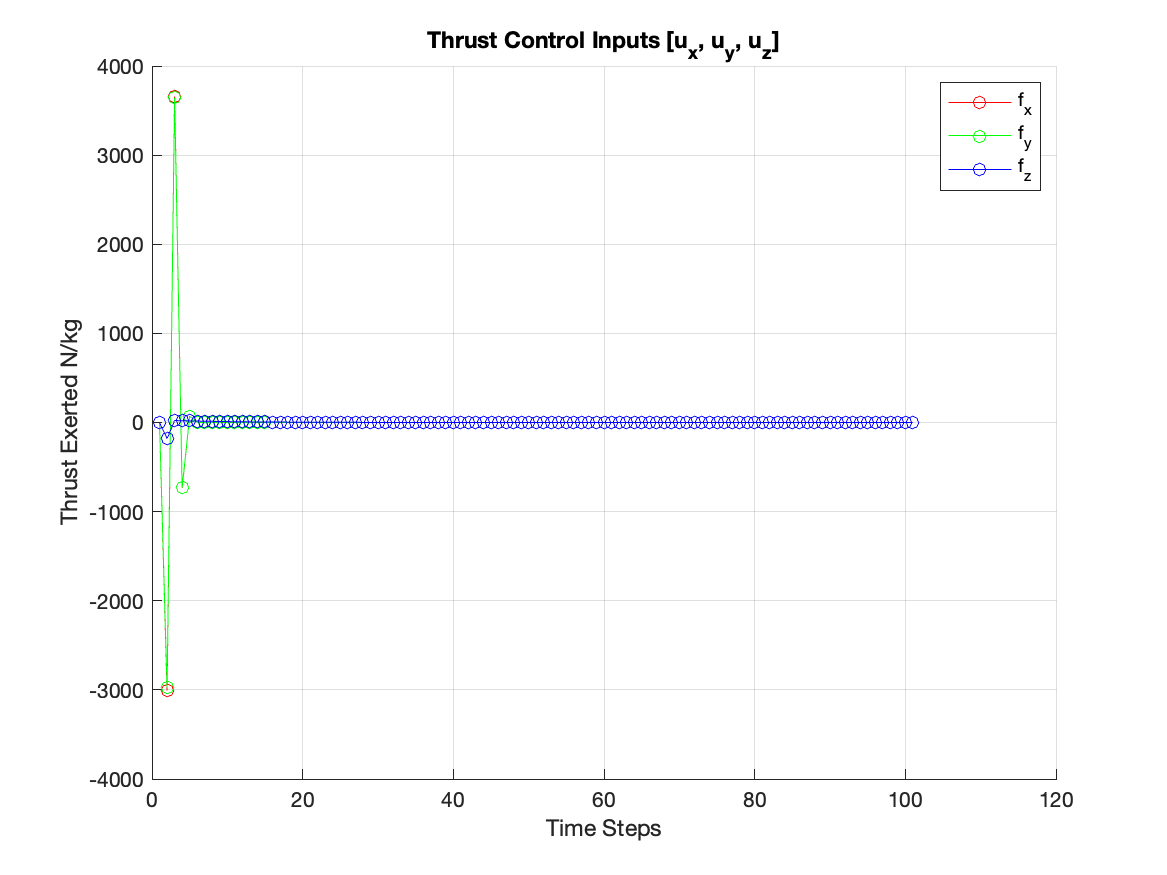
\includegraphics[width=\columnwidth]{new_final_figs/Unconstrained_input_plot.png}
        \caption{Unconstrained Thrust Control Input}
        \label{unconst:control_in}
    \end{subfigure}
    \begin{subfigure}{\columnwidth}
        \centering
        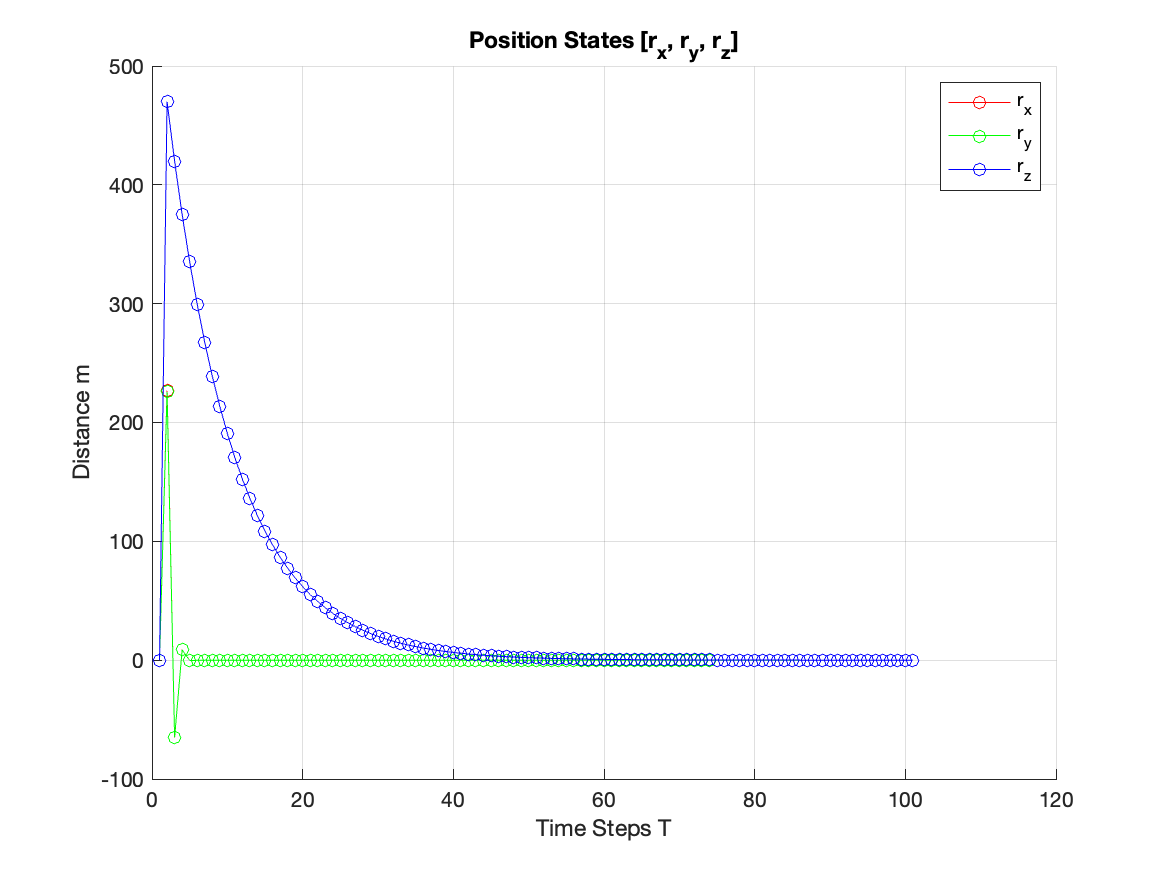
\includegraphics[width=\columnwidth]{new_final_figs/Unconstrained_position_state_plot.png}
        \caption{Unconstrained Position State Plot}
        \label{unconst:pos_state}
    \end{subfigure}
    \begin{subfigure}{\columnwidth}
        \centering
        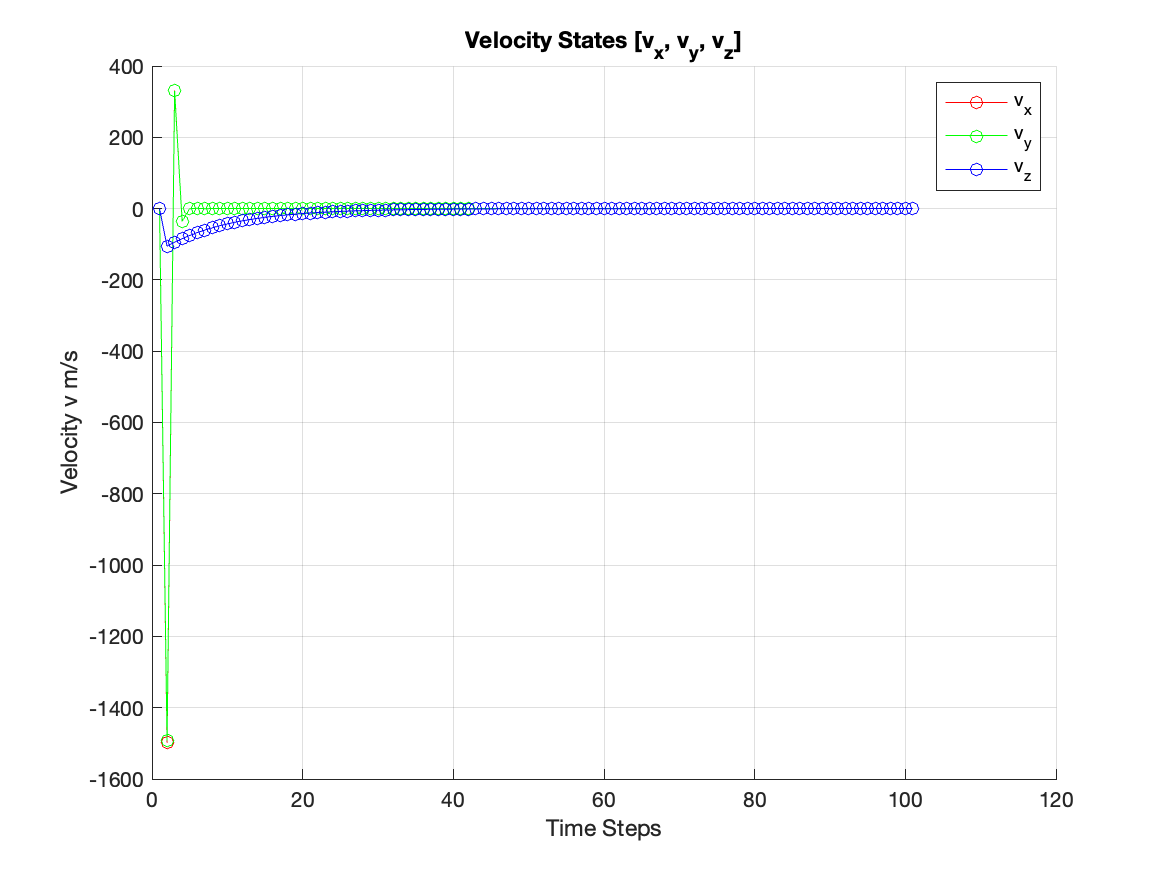
\includegraphics[width=\columnwidth]{new_final_figs/Unconstrained_velocity_state_plot.png}
        \caption{Unconstrained Velocity State Plot}
        \label{unconst:vel_ss}
    \end{subfigure}
\end{figure}


\subsection{Constrained}
\begin{figure}[H]
    \centering
    \begin{subfigure}{\columnwidth}
        \centering
        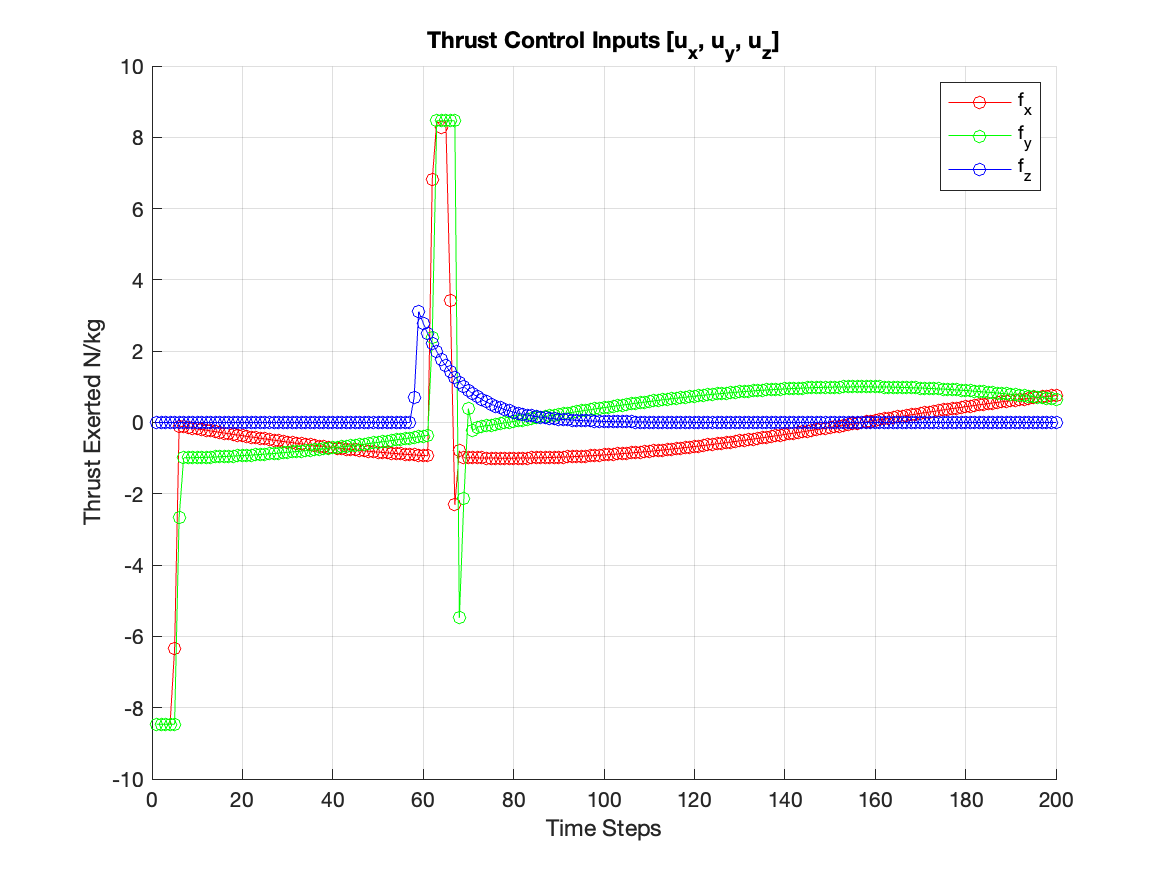
\includegraphics[width=\columnwidth]{new_final_figs/Constrained_input_plot.png}
        \caption{Constrained Thrust Control Input}
        \label{const:control_in}
    \end{subfigure}
    \begin{subfigure}{\columnwidth}
        \centering
        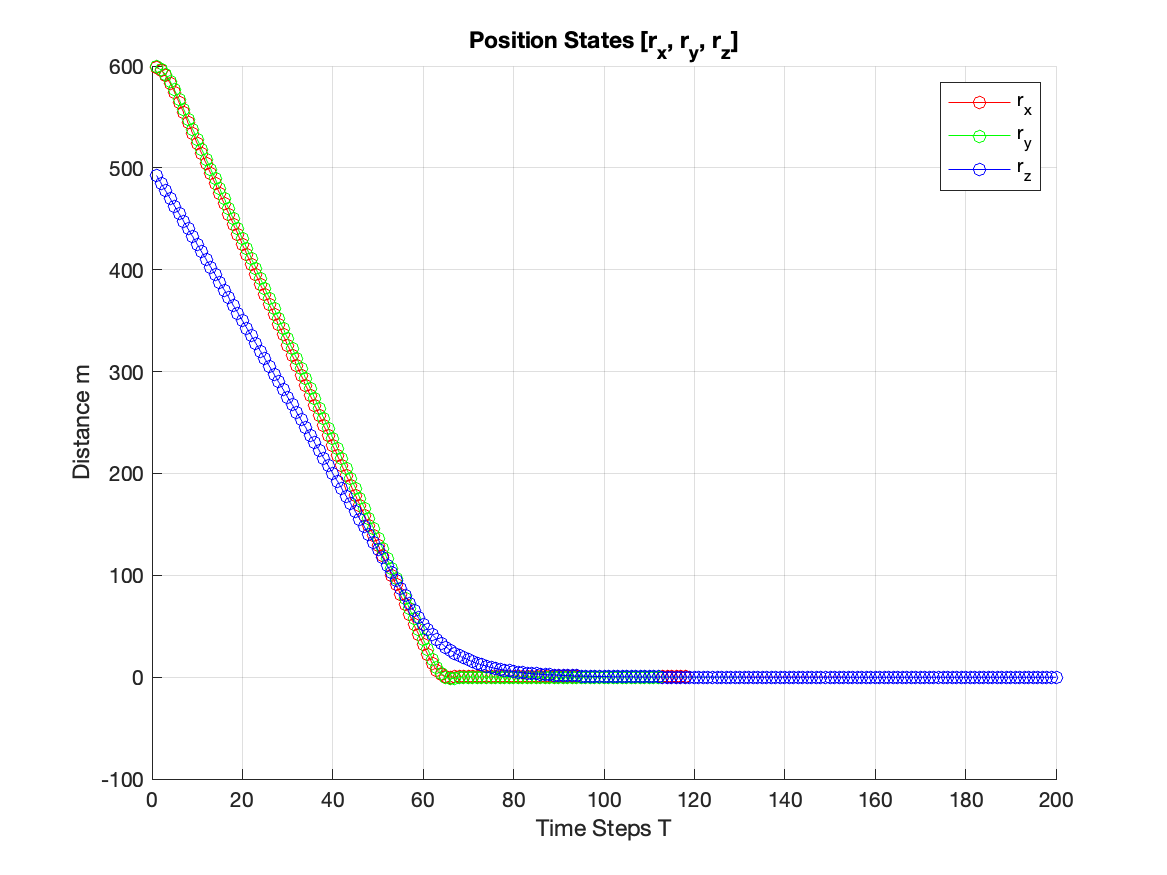
\includegraphics[width=\columnwidth]{new_final_figs/Constrained_position_state_plot.png}
        \caption{Constrained Position State Plot}
        \label{const:pos_state}
    \end{subfigure}
    \begin{subfigure}{\columnwidth}
        \centering
        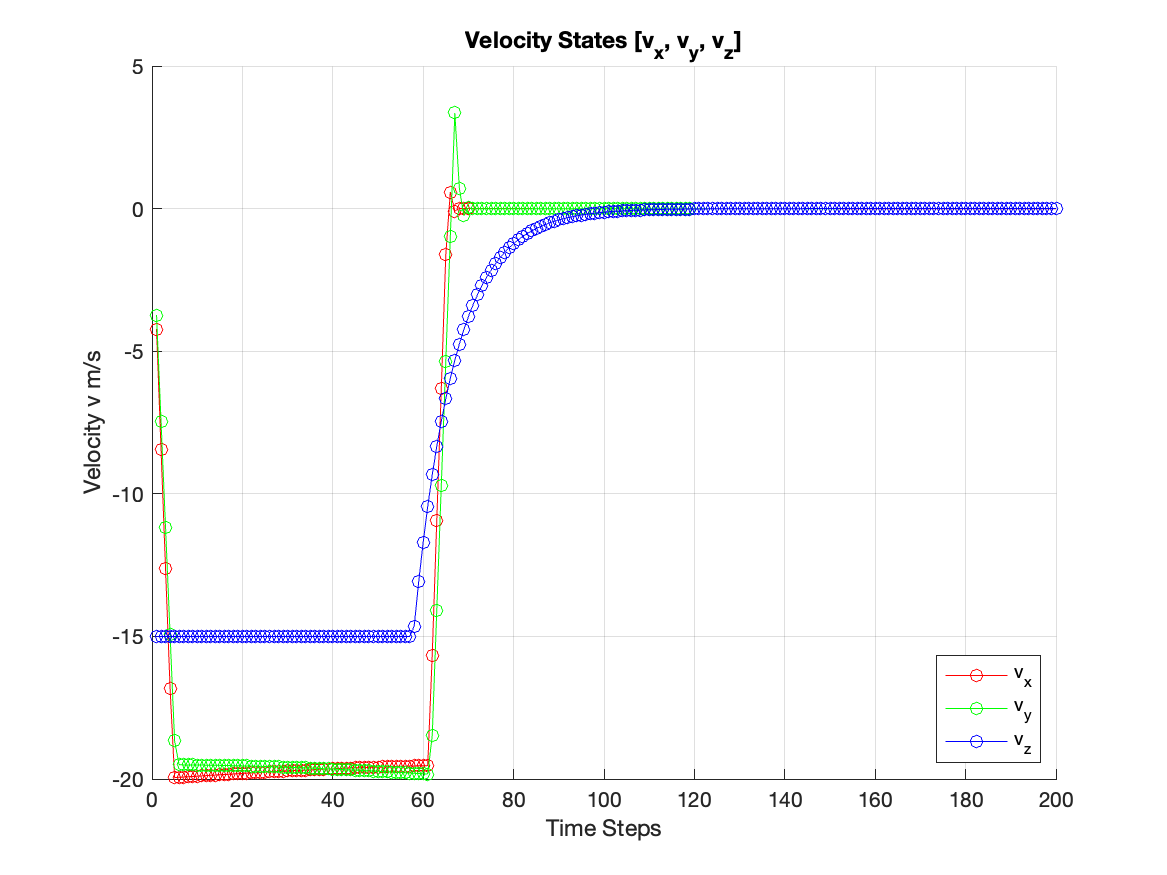
\includegraphics[width=\columnwidth]{new_final_figs/Constrained_velocity_state_plot.png}
        \caption{Constrained Velocity State Plot}
        \label{const:vel_ss}
    \end{subfigure}
\end{figure}
\subsection{Disturbance Rejection}
\begin{figure}[H]
    \centering
    \begin{subfigure}{\columnwidth}
        \centering
        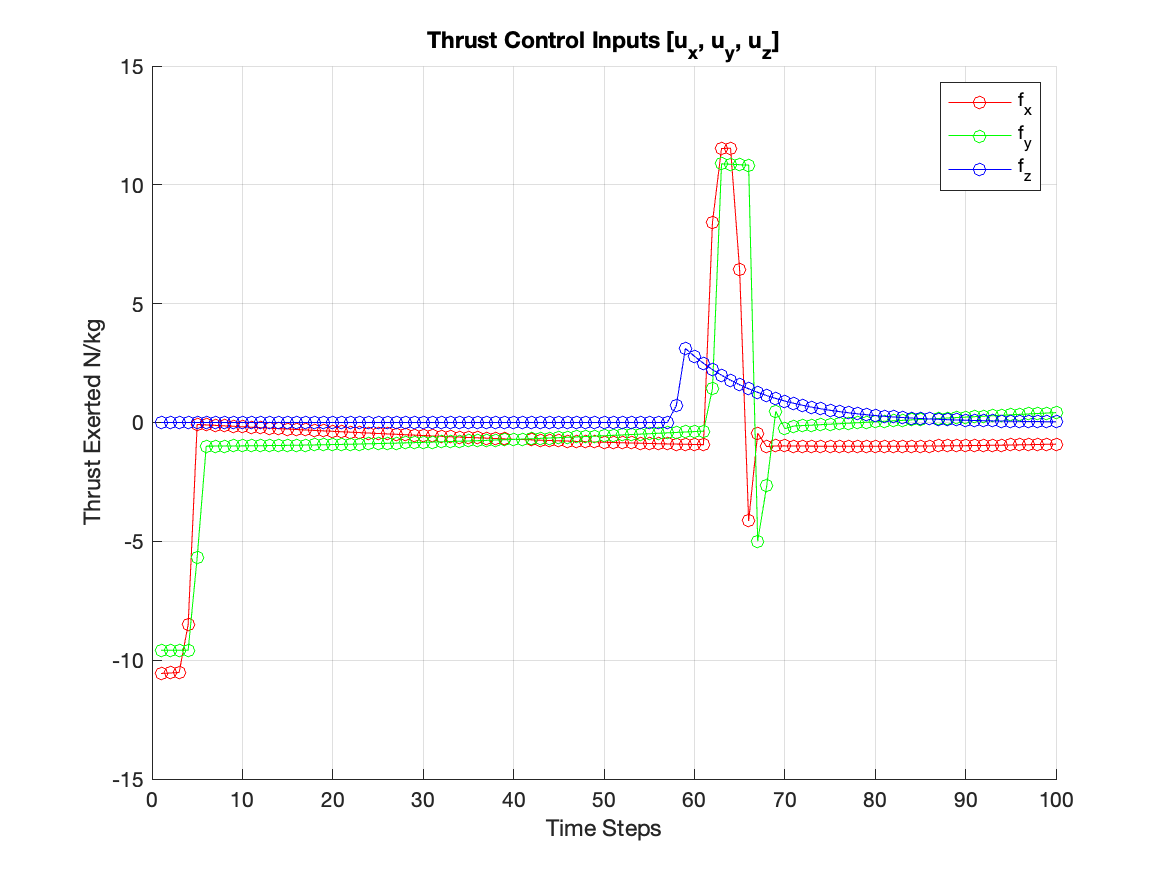
\includegraphics[width=\columnwidth]{new_final_figs/DR_Constrained_input_plot.png}
        \caption{Disturbance Rejection Thrust Control Input}
        \label{DR:control_in}
    \end{subfigure}
    \begin{subfigure}{\columnwidth}
        \centering
        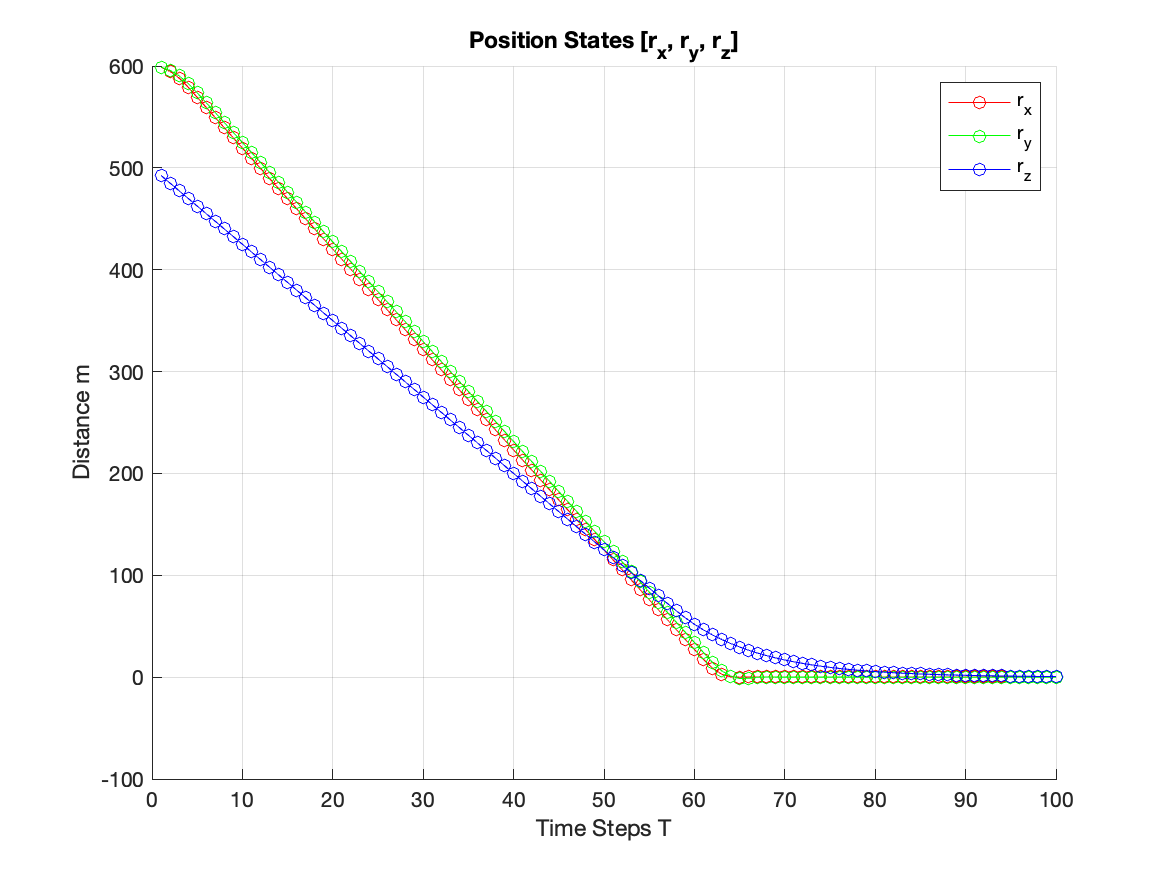
\includegraphics[width=\columnwidth]{new_final_figs/DR_Constrained_position_state_plot.png}
        \caption{Disturbance Rejection Position State Plot}
        \label{DR:pos_state}
    \end{subfigure}
    \begin{subfigure}{\columnwidth}
        \centering
        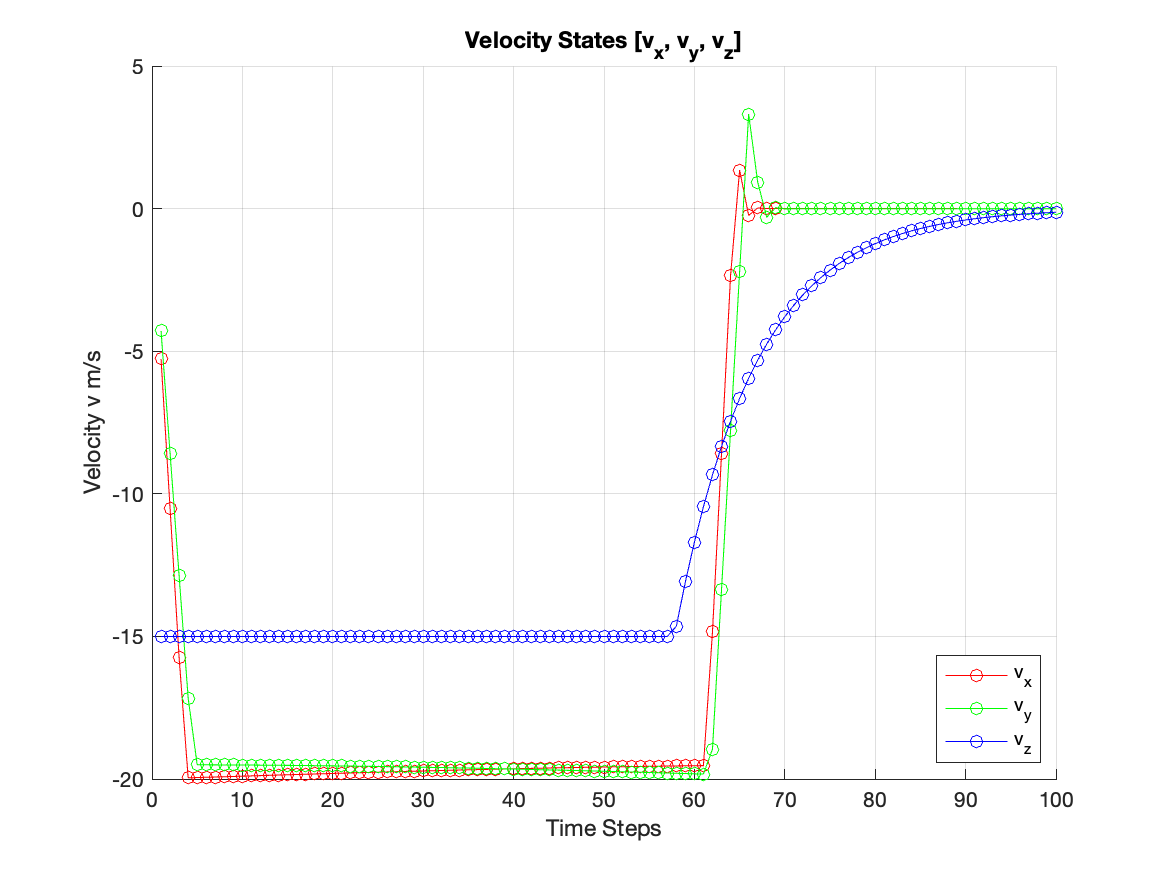
\includegraphics[width=\columnwidth]{new_final_figs/DR_Constrained_velocity_state_plot.png}
        \caption{Disturbance Rejection Velocity State Plot}
        \label{DR:vel_ss}
    \end{subfigure}
\end{figure}

\section{Analysis \& Discussion}
Due to the limitations to the number of pages, the analysis will mainly discuss the effectiveness of the controllers using constraints and disturbance rejection. \\


\section{Conclusion}


\newpage

\bibliographystyle{ieeetr} % Add the bibliography style
\bibliography{references.bib}

\appendix

\section{A}


\end{document}
